
% The system takes a real-time stream of think-aloud utterances from a VR session and produces an IPQ score at the item, subscale, and total level for that session (see Figure~\ref{fig:teaser}).
% It is organized as a two-stage front-end classifier that sorts each utterance, followed by a multi-agent scoring chain that turns the sorted utterances into IPQ scores.
% An evidence gate is applied inside the scoring chain, not at the front end: the front end decides where an utterance is routed, and the gate decides whether the routed utterances actually support a rated item.
% The word ``gate'' in the paper title refers to this scoring-stage evidence gate.
% The system produces per-item, per-subscale, and total IPQ scores for a session; items for which no supporting evidence is found are left missing; no value is imputed.




% \subsection{Overview}

\section{Proposed LLM-Based System for Quantifying Presence from Think-Aloud Utterances}
\label{sec:system}


\hsnote{The proposed system takes think-aloud utterances collected during a VR experience as input and converts them into quantitative presence scores based on the IPQ (Figure~\ref{fig:teaser}). The system consists of two main stages: an utterance-classification stage that identifies and routes presence-related verbalizations, followed by a multi-agent scoring stage that evaluates the routed utterances according to the corresponding IPQ items.} 
\vsnote{The front-end classifier was developed using an anonymized, human-labeled corpus collected in prior studies, providing domain-specific examples of how users verbally express presence-related experiences. The anonymized dataset will be made publicly available following publication.} 

\hsnote{Within the scoring stage, an evidence gate determines whether the available utterances provide sufficient support for rating each IPQ item. Thus, the classification stage determines which IPQ dimensions an utterance may relate to, whereas the evidence gate determines whether the available verbal evidence is sufficient to produce a score. Based on the accepted evidence, the system generates item-level scores, which are subsequently aggregated into IPQ subscale and overall presence scores. When no supporting evidence is available for an item, the corresponding score is left missing rather than imputed.}
\vsnote{This separation distinguishes whether an utterance is potentially relevant to a presence construct from whether it contains sufficient evidence to justify a quantitative IPQ score.}


The 14 IPQ items, their subscales, and the response anchors used in this study are listed in Appendix~\ref{sec:appendix} (Table~\ref{tab:ipq_items}).



\subsection{Front-End Routing Classifier and Training Data} 

% The front end is a locally fine-tuned small language model that assigns each incoming utterance one of five categories: GP, SP, INV, REAL, or NONE.
% Its purpose is routing, not scoring: it selects which utterances the downstream scoring chain should consider for which subscale.
% The deployed configuration combines the fine-tuned adapter with a keyword layer that raises recall on rare categories at the cost of some precision.
% On a held-out set of 73 utterances, the deployed configuration reached a macro $F_1$ of $0.567$, up from $0.400$ for the adapter alone.
% An alternative retrained adapter was evaluated and not adopted because it lost recall on SP and produced a lower combined macro $F_1$ (see Section~\ref{subsec:rq2}).
% The classifier runs on-device so that participants' raw speech does not leave the local machine at this stage.


% The front-end classifier was developed using an anonymized corpus collected in prior studies. The corpus contained 823 human-labeled records derived from 551 unique utterances. Because a single utterance could be associated with more than one presence-related construct, utterances with multiple labels contributed multiple label records after multi-label expansion. An additional 72 synthetic examples were generated for General Presence (GP), which was comparatively underrepresented in the original corpus. A separate silver-labeled dataset was excluded from model development because its estimated labeling error rate was 29\%. The anonymized dataset used for developing the classifier will be made publicly available following publication to support reproducibility and future research.


The front-end classifier was developed using an anonymized corpus collected in prior studies, consisting of 823 human-labeled records derived from 551 unique utterances. Because an utterance could be associated with more than one presence-related construct, multi-label utterances contributed multiple label records. To supplement the relatively underrepresented General Presence (GP) category, 72 synthetic examples were added to the training data. A separate silver-labeled dataset was excluded because its estimated labeling error rate was 29\%. The anonymized dataset will be made publicly available following publication.

The human-labeled corpus was partitioned by utterance ID using a hash-based 80/10/10 split into training, validation, and held-out test sets, with all synthetic examples restricted to the training set. The held-out test set contained 73 label records corresponding to 37 unique human utterances that were not used for model training.

The front end employs EXAONE 2.4B, locally fine-tuned using QLoRA-based parameter-efficient fine-tuning, to classify each incoming think-aloud utterance into GP, SP, INV, REAL, or NONE. Its purpose is routing rather than scoring: the classifier determines which utterances should be forwarded to the downstream multi-agent scoring chain and which IPQ dimension they may provide evidence for.

The deployed configuration combines the fine-tuned adapter with a keyword-based layer to improve recall for relatively sparse presence categories. On the held-out test set, this configuration achieved a macro $F_1$ of $0.567$, compared with $0.400$ for the adapter alone. The routing classifier runs locally on the experimental machine, so participants' raw speech does not leave the local environment at this stage.


\subsection{Multi-Agent Scoring Chain and Evidence Gate}

Utterances routed to one or more presence-related categories are passed to a multi-agent scoring chain consisting of three functional roles: Drafter, Reviewer, and Rater (Figure~\ref{fig:pipeline_example}). The Drafter identifies item-level evidence for the 14 IPQ items from the routed think-aloud utterances. The Reviewer then examines the proposed evidence and accepts, edits, or rejects it. Based on the reviewed evidence, the Rater assigns a score from 0 to 6 to each supported IPQ item; items with rejected or absent evidence are left missing. Reverse-keyed items (SP2, INV3, and REAL1) are scored in their original direction and reversed during aggregation.

An evidence gate operates between the Reviewer and Rater. Thus, routing an utterance to an IPQ dimension does not necessarily result in a score; an item is rated only when sufficient verbal evidence is identified and accepted.

Each IPQ item is accompanied by an item card specifying the verbal cues that can serve as evidence for that item. The cards include sub-indicators, boundary rules for neighboring items, and brief scoring guidance, and are provided as fixed reference text in the Drafter and Rater prompts. A relation graph among IPQ items further supports the Drafter and Reviewer in distinguishing conceptually related items. The development of these item cards and the corresponding ablation analyses are reported in Section~\ref{subsec:ablation}.


% Utterances that the front end routes to 
% a construct category enter a scoring chain composed of three functional roles (Figure~\ref{fig:pipeline_example}).
% A drafter agent proposes item-level evidence for the 14 IPQ items using the routed utterances as input.
% A reviewer agent then inspects the proposed evidence and either accepts, edits, or rejects it, functioning as an independent second reader.
% A rater agent assigns a $0$--$6$ score for each item for which reviewed evidence was accepted; items whose evidence is rejected or absent are marked missing.
% Reverse-keyed items (SP2, INV3, REAL1) are rated on the original polarity and reversed at aggregation.
% The evidence gate operates between the reviewer and the rater: only items backed by the accepted evidence produce a rated score.
% \redout{This rule is what the paper title's ``evidence-gated'' refers to, and it is applied consistently across every session.}

% Each of the 14 items has a card that states what counts as evidence for it: sub-indicators (the cues a speaker might voice), boundary rules against neighboring items, and a short guide paragraph. The cards are placed in the drafter's and rater's prompts as fixed reference text, so the drafter looks for the same cues and the rater scores against the same definitions in every session; a relation graph between items gives the drafter and reviewer a hint about which neighboring item a cue may belong to. The cards' development, an ablation that removes them on 12 sessions, the keyword layer's contribution, and the discarded scoring-stage alternatives are reported in Section~\ref{subsec:ablation}.

\subsection{Aggregation and Score Definition}

Because an IPQ item may receive scores from multiple think-aloud utterances during a session, the system first generates utterance-level item scores and then aggregates them into a single session-level score for each item. When multiple scores are available for the same item, the 75th percentile is used as the session-level item score. Reverse-keyed items are reversed before aggregation.

Each IPQ subscale score is calculated as the mean of the scored items within that subscale. The overall presence score is calculated as the mean of all scored IPQ items available for the session.

If no sufficient verbal evidence is identified for an item, the item is retained as missing. Missing items are neither treated as zero nor imputed and are excluded from the corresponding subscale and overall score calculations. Thus, a missing value indicates insufficient think-aloud evidence for rating the item, rather than low presence.

Figure~\ref{fig:pipeline_example} illustrates this process by tracing a representative think-aloud utterance from routing and evidence identification to item-level scoring and session-level aggregation.





\begin{figure*}[t]
\centering

\includegraphics[width=\textwidth]{Figures/Workflow_Example.png}
\caption{One utterance traced through the scoring chain to a session score (participant PT001, \textit{Half-Life: Alyx}, 01:14). Panels 1--5 show routing, drafted cues, the reviewer and evidence gate, and the rater's item scores; panel 6 shows the session-level values, where an item scored by several utterances takes the 75th percentile, each subscale is the mean of its scored items, and the total is the mean of all scored items. Hatched cells are items with no accepted evidence and are left missing rather than imputed. The lower branch shows where scores are lost: (a) an utterance with drafted cues for which the rater returned no score, and (b) INV1 and INV3, which are scored from the absence of a signal and therefore carry no sub-indicator marked present.}
\Description{A six-stage flow diagram read left to right. Stage one shows a speech bubble with the utterance and the participant, game, and time. Stage two shows the on-device classifier box labeled EXAONE 2.4B plus QLoRA with the output tag GENERAL SP. Stage three shows six item cards from the drafter: GP1 with two cues, SP1 with one, SP2 with two, SP3 with one, SP5 with two, and SP4 with no cue. Stage four shows a reviewer box and a vertical evidence gate; five arrows pass through and the SP4 arrow stops at a box labeled missing. Stage five lists the rater scores GP1 5, SP1 4, SP2 raw 1.5 reversed to 4.5, SP3 4.5, SP5 5. Stage six shows a grid of the fourteen IPQ items with session values, hatched cells for the four missing items SP4, INV1, INV2, INV3, the subscale means GP 5.75, SP 4.59, INV 3.40, REAL 2.58, and the total 3.78 next to the self-report total 4.50. Below the flow, a side branch labeled where scores are lost shows a second utterance whose REAL1 and REAL3 cues received no score, and a note that INV1 and INV3 are scored from the absence of a signal and cannot pass the gate.}
\label{fig:pipeline_example}
\end{figure*}




\subsection{\hsnote{Post-Scoring Review Module}}



\hsnote{A review module was developed to inspect the outputs generated by the automated scoring pipeline (Figure~\ref{fig:interface}). For each rated IPQ item, the interface presents the assigned score together with the supporting think-aloud utterance and the corresponding time-stamped playback of the VR session. This allows a reviewer to check the contextual evidence behind each score. By linking each quantitative score back to the original utterance and its corresponding VR context, the interface enables direct inspection of how the automated system reached its judgment.}

The module does not alter scores; every score reported in this paper is the pipeline's unmodified output. Thus, the module functions as an audit and interpretation tool rather than as a human-in-the-loop correction stage.


\hsnote{The module also supports retrospective inspection of how a session-level score was constructed, as each rated item is linked to the timestamp of the utterance that provided its evidence. 
The interface was used for auditing the scored sessions. Figure~\ref{fig:interface} shows the interface for a TAP session (a) and a non-TAP (Control) session (b).}



\begin{figure*}[t]
\centering
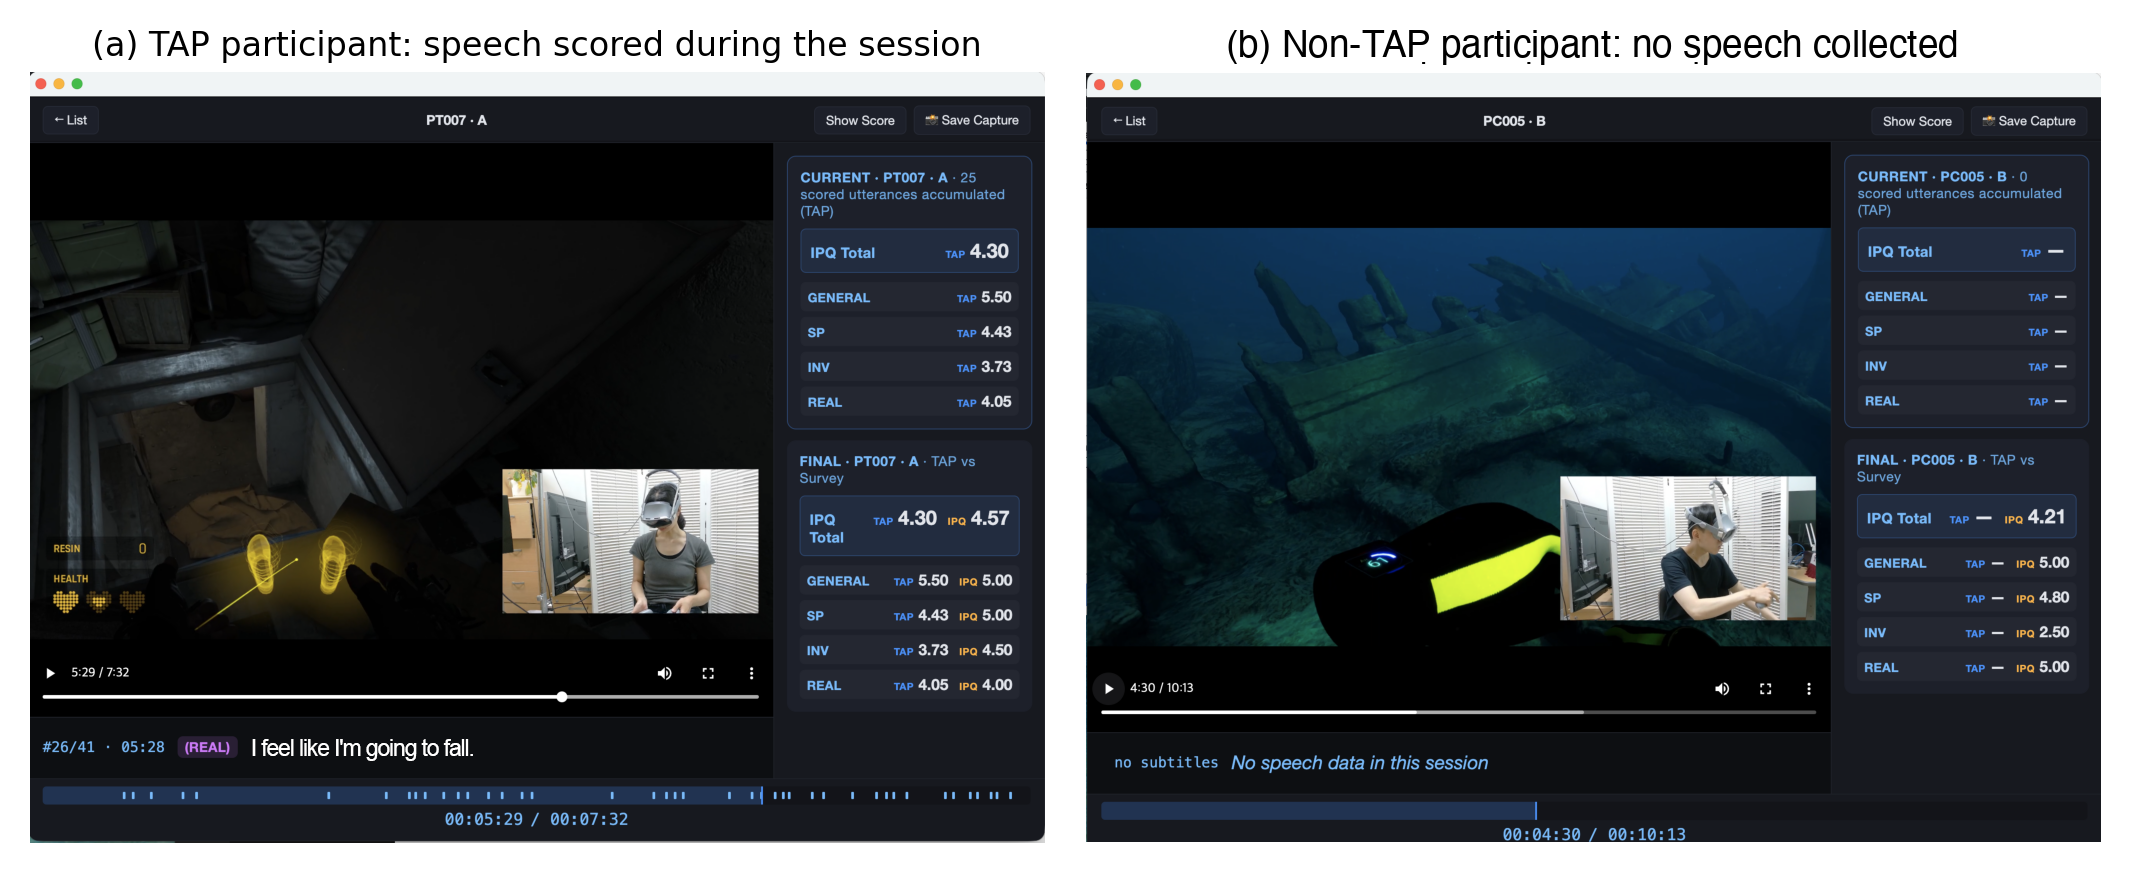
\includegraphics[width=\textwidth]{Figures/F12_viewer_PT_vs_PC.png}
\caption{The analysis interface on a TAP session (a) and a Non-TAP session (b). 
In (a), the panel shows the game view with the participant's webcam inset, the current utterance with the construct the front end routed it to, the utterance timeline with its construct markers, and the running speech-derived IPQ scores beside the self-reported ones. 
In (b), no speech was collected by design, so the utterance track is empty and every speech-derived field is blank while the questionnaire scores remain.}
\Description{Two screenshots of the review application side by side. The left shows a think-aloud session with a subtitle line, construct markers along a timeline, and speech-derived scores. The right shows a non-TAP session with no subtitles, an empty timeline, and dashes in place of the speech-derived scores.}
\label{fig:interface}
\end{figure*}



\begin{figure*}[t]
\centering

\includegraphics[width=\textwidth]{Figures/F03_console.png}
\caption{Experimental setup. \textcircled{\scriptsize 1} Play area: the participant's chair in front of the webcam. \textcircled{\scriptsize 2} Operator console (bottom) and gate monitor with running per-category utterance counts (top). \textcircled{\scriptsize 3} Coverage indicator shown in the headset during the practice session only, hidden in all experimental sessions: four boxes naming the IPQ constructs with example expressions. \textcircled{\scriptsize 4} Real-time transcription window: each recognized utterance with the category assigned by the local front-end classifier and the accumulated cost; from here the operator releases the session to the post-session scoring workflow. \note{korean language needs to be changed}}
\Description{Four panels side by side: a photograph of a chair in a laboratory; a dark operator console with a gate monitor showing five category counters; a virtual reality view with four labeled text boxes for General Presence, Spatial Presence, Involvement, and Experienced Realism; and a transcription log listing Korean utterances with category tags.}
\label{fig:console}
\end{figure*}




% [MCd 2026-09-11] 제목의 "and Refinement" 제거. 리뷰 앱은 점수 편집 기능이 없음 (apps/review-app: 통합기록 xlsx 점수를 읽어 표시만 함). 교수님 문면의 "manually revise the assigned score" 는 2765111 원문 오타 "it does make, alter or adjust the scores" (not 누락) 를 그대로 읽은 결과임. 논문 점수는 전부 파이프라인 산출 그대로.

% The diagram layout was drafted with Gemini image generation from the authors' written specification and redrawn by the authors; every utterance, cue count, score, and aggregate shown is taken from the deployed pipeline's logs.




% An analysis module, developed for post-hoc inspection, aligns and presents each rated item with the utterance that produced its evidence and with the corresponding time-stamped playback of the VR session 
% (see Figure~\ref{fig:interface}). 
% This module is used only for auditing and vignette construction (see Section~\ref{subsec:vignettes}); it does
% [MCd 2026-09-11] 아래 원문 줄은 "it does NOT make, alter or adjust the scores" 의 오타 (not 누락). 교수님 "manually revise" 문장의 출처. 본문은 ②로 정정됨.
% make, alter or adjust the scores.
% Because every rated item carries the timestamp of the utterance that supplied its evidence, it replays how a session score was reached (Section~\ref{subsec:rq1_within}). Figure~\ref{fig:interface} shows the interface at one moment of a think-aloud session (a) and of a control session (b).